\documentclass[12pt,a4paper,oneside]{book}

% --------------------------------- 페이지 스타일 지정
	\usepackage{geometry}
	\geometry{top=1.4in}
	\geometry{bottom=1.4in}
	\geometry{left=1.2in}
	\geometry{right=1.2in}
	\geometry{headheight=0.4in}
	\geometry{headsep=0.1in}
	\geometry{footskip=0.3in}
%	\geometry{showframe}
	
	\newgeometry{ 	top=8em, bottom=8em,
					left=8em, right=8em, 
					headheight=2em, headsep=2em}


%		\usepackage[hangul]{kotex}				% 한글 사용
		\usepackage{kotex}						% 한글 사용
		\usepackage[unicode]{hyperref}			% 한굴 하이퍼링크 사용
		\usepackage{amssymb,amsfonts,amsmath}% 수학 수식 사용
		\usepackage{scrextend}					% 
		
		
		\usepackage{enumerate}			%
		\usepackage{enumitem}			%
		\usepackage{longtable}			%

		\usepackage{pifont}				%
		\usepackage{setspace}			%
		\usepackage{booktabs}			% table
		\usepackage{color}				%
		\usepackage{multirow}			%
		\usepackage{boxedminipage}		% 미니 페이지
		\usepackage[pdftex]{graphicx}	% 그림 사용
		\usepackage[final]{pdfpages}	%pdf 사용
		\usepackage{framed}			%pdf 사용
		
		\usepackage{fix-cm}	
		\usepackage[english]{babel}

		\usepackage{tikz}%
		\usetikzlibrary{arrows,positioning,shapes}
		%\usetikzlibrary{positioning}
		
		\usepackage{blindtext}





% --------------------------------- 페이지 스타일 지정

	\usepackage[Bjornstrup]{fncychap}

	\usepackage{fancyhdr}
	\pagestyle{fancy}
	\fancyhead{} % clear all fields
	\fancyhead[LO]{\tiny \leftmark}
	\fancyhead[RE]{\tiny \leftmark}
	\fancyfoot{} % clear all fields
	\fancyfoot[LE,RO]{\large \thepage}
	%\fancyfoot[CO,CE]{\empty}
	\renewcommand{\headrulewidth}{1.0pt}
	\renewcommand{\footrulewidth}{0.4pt}
	
	
	
% --------------------------------- section 스타일 지정

	\usepackage{titlesec}
	
	\titleformat*{\section}{\large\bfseries}
	\titleformat*{\subsection}{\normalsize\bfseries}
	\titleformat*{\subsubsection}{\normalsize\bfseries}
	\titleformat*{\paragraph}{\normalsize\bfseries}
	\titleformat*{\subparagraph}{\normalsize\bfseries}

	\renewcommand{\thesection}{\arabic{section}.}
	\renewcommand{\thesubsection}{\thesection\arabic{subsection}.}
	\renewcommand{\thesubsubsection}{\thesubsection\arabic{subsubsection}}
	
	\titlespacing*{\section} 		{0pt}{0.0em}{0.0em}
	\titlespacing*{\subsection}	  	{0ex}{0.0em}{0.0em}
	\titlespacing*{\subsubsection}	{0ex}{0.0em}{0.0em}
	\titlespacing*{\paragraph}		{0ex}{0.0em}{0.0em}
	\titlespacing*{\subparagraph}	{0ex}{0.0em}{0.0em}

%	\titlespacing*{\section} 		  	{0pt}{0.0\baselineskip}{0.0\baselineskip}
%	\titlespacing*{\subsection}	  	{0ex}{0.0\baselineskip}{0.0\baselineskip}
%	\titlespacing*{\subsubsection}	{6ex}{0.0\baselineskip}{0.0\baselineskip}
%	\titlespacing*{\paragraph}		{6pt}{0.0\baselineskip}{0.0\baselineskip}
	
	
% ----------------------------- 장의 목차
\usepackage{minitoc}
	\setcounter{minitocdepth}{1}    	% Show until subsubsections in minitoc
	\setlength{\mtcindent}{12pt} 	% default 24pt
	
	
% --------------------------------- 문서 기본 사항 설정
		\setcounter{secnumdepth}{3} % 문단 번호 깊이
		\setcounter{tocdepth}{3} % 문단 번호 깊이
		\setlength{\parindent}{0cm} % 문서 들여 쓰기를 하지 않는다.
		\doublespace

% --------------------------------- recoment
		\renewcommand{\labelitemi}{$\bullet$}
		\renewcommand{\labelitemii}{$\cdot$}
		\renewcommand{\labelitemiii}{$\diamond$}
		\renewcommand{\labelitemiv}{$\ast$}		
	
% ------------------------------------------------------- enumi setting
%		\renewcommand{\labelenumi}{\arabic{enumi}.} 
%		\renewcommand{\labelenumii}{\arabic{enumi}.\arabic{enumii}}
		\renewcommand{\labelenumii}{(\arabic{enumii})}
		\renewcommand{\labelenumiii}{\arabic{enumiii})}
%		\setlist{itemsep=0.0em}
		\setlist[enumerate,1]{labelindent=0.0em,leftmargin=8.0ex,rightmargin=2.0em,}
		\setlist[enumerate,2]{labelindent=0.0em,leftmargin=4.0ex,rightmargin=2.0em,}
		\setlist[enumerate,3]{labelindent=0.0em,leftmargin=3.0ex,rightmargin=2.0em,}
%		\setlist[enumerate,1]{label=\arabic*., ref=\arabic*}
%		\setlist[enumerate,2]{label=\emph{\alph*}),ref=\theenumi.\emph{\alph*}}
%		\setlist[enumerate,3]{label=\roman*), ref=\theenumii.\roman*}

% --------------------------------- recoment

	\newcommand{\red}{\color{red}}			% 글자 색깔 지정
	\newcommand{\blue}{\color{blue}}		% 글자 색깔 지정
	\newcommand{\black}{\color{black}}		% 글자 색깔 지정
	\newcommand{\superscript}[1]{${}^{#1}$}
	
	
% --------------------------------- 환경 정의 : 박스 치고 안의 글자 빨간색

			\newenvironment{BoxRedText}
			{ 	\setlength{\fboxsep}{12pt}
				\begin{boxedminipage}[c]{1.0\linewidth}
				\color{red}
			}
			{ 	\end{boxedminipage} 
				\color{black}
			}
			
%		\setmainhangulfont[BoldFont=HY견고딕]{한컴돋움}
%		\setsanshangulfont{HY견고딕}
%		\setmonohangulfont{한컴돋움}
			
			

% ------------------------------------------------------------------------------
% Begin document (Content goes below)
% ------------------------------------------------------------------------------
	\begin{document}
	
			\dominitoc
			

			\title{typing}
			\author{김대희}
			\date{2015년 1월}
			\maketitle


			\tableofcontents
			\listoffigures
			\listoftables

			


% \\\\\\\\\\\\\\\\\\\\\\\\\\\\\\\\\\\\\\\\\\\\\\\\\\\\\\\\\\\\\\\\\\\\\\\\\\\\\  Part

		\part{part1}

% ========================================== part      ============
		\part[실행단계 Post-Syudy Phase]{실행단계 \\ Post-Syudy Phase}

% ========================================== chapter ============
\newpage
\chapter{chapter name}

	% -------------------------------------- page -------------------
	%	\nomtcrule         		% removes rules = horizontal lines
	%	\nomtcpagenumbers  % remove page numbers from minitocs
		\newpage
		\minitoc				% Creating an actual minitoc
	%	\doublespace

% ------------------------------------------ section ------------ 
\newpage  \null
\section{LCC 개요}






% ------------------------------------------ section ------------ 
\newpage
\section{LCC 개요}

	\subsection{중점 품질 관리대상}

		\subsubsection{중점 품질 관리대상}

		\paragraph{중점 품질 관리대상}

		\subparagraph{중점 품질 관리대상}

%		\Blinddocument
				
		\newpage   \null
	% -------------------------------------- page -------------------
		\subsection{중점 품질 관리대상}
		
		\newpage
	% -------------------------------------- page -------------------
	\newpage
	\paragraph{\large }

% \\\\\\\\\\\\\\\\\\\\\\\\\\\\\\\\\\\\\\\\\\\\\\\\\\\\\\\\\\\\\\\\\\\\\\\\\\\\\  Part

		\addtocontents{toc}{\protect\newpage}
		\part{part1}
		
% ========================================== chapter ============
\newpage  \null
\chapter{공사 착수 단계}
\null

				
% ========================================== chapter ============
\newpage
\chapter{폰트 테스트}

		\begin{itemize}
		\item \textrm{\huge serif(main)은 `서울한강L(한글)'과 `Constantia'(영문)}
		\item \textrm{\huge serif의 漢字는 `함초롬 바탕 LVT'}
		\item \textsf{\huge sans serif는 `a고래야놀자(한글)'과 `Chinacat'(영문)}
		\item \texttt{\huge typewriter는 `a하늘산책M(한글)'과 `The Great Escape'(영문)}
		\end{itemize}

% ========================================== chapter ============
\newpage
\chapter{List}
\newpage  \null

	% ==============================================================================	
	%  																			List
	% ==============================================================================	

		% ----------------------------- itemize
			\begin{itemize}[itemsep=0.0em]
			\item	
			\end{itemize}
			
			\begin{itemize}[topsep=0.0em,itemsep=0.0em]
			\item	
			\end{itemize}	


			[itemsep=-0.5em]
			[topsep=-1.0em,			]


			\begin{itemize}[	topsep=0.0em,itemsep=0.0em,
							leftmargin=4em, labelsep=3em ]
			\item	
			\end{itemize}	

			
		% ----------------------------- itemize
		\def\TStart{	\setlength{\fboxsep}{12pt}
					\begin{boxedminipage}[c]{1.0\linewidth}
					\begin{itemize}[topsep=0.0em,itemsep=0.0em]
					}
		\def\TEnd{	\end{itemize}	
					\end{boxedminipage}\\
					}
		\TStart
		\item 1 
		\item 2 
		\TEnd

		\setlength{\fboxsep}{12pt}
		\begin{boxedminipage}[c]{1.0\linewidth}
		\end{boxedminipage}\\


		% ----------------------------- enumerate
		\begin{enumerate}[itemsep=0.0em]
		\item	
		\item	
		\end{enumerate}
		
		% ----------------------------- enumerate
		\begin{enumerate}[ topsep=0.0em, itemsep=-0.5em ]
		\item	
		\item	
		\end{enumerate}
		
		% ----------------------------- enumerate
		\begin{enumerate}[ label=\arabic*), topsep=-1.0em, itemsep=-0.5em ]
		\item	
		\end{enumerate}

		% ----------------------------- enumerate
		\begin{enumerate}[ 	label=\arabic*), 
							topsep=-1.0em, itemsep=-0.5em,
							leftmargin=4em, labelsep=3em ,
							labelwidth=0.0em]
		\item	
		\end{enumerate}

		% ----------------------------- enumerate
		\begin{enumerate}[ 	topsep=0.0em, itemsep=0.0em,
							leftmargin=4em, labelsep=3em ,
							labelwidth=0.0em]
		\item	
		\end{enumerate}



		\begin{dingautolist}{172}
		\item	보강토체를 따른 활동(성토체내의 흙과 흙 사이의 내부마찰각) 
		\item	기초지반을 따른 활동(성토체흙과 기초지반흙과의 마찰각) 
		\item	최하단 토목섬유 보강재와 흙 사이의 경계면을 따른 활동 
		\end{dingautolist}

		

	% ----------------------------- boxed mini page
		\setlength{\fboxsep}{12pt}
		\begin{boxedminipage}[c]{1.0\linewidth}
		\end{boxedminipage}\\
		
		\begin{framed}
		1
		\end{framed}
		
		\begin{quote}
		“         ”
		\end{quote}
		
		\begin{verbatim}
		\end{verbatim}

		
		\rule{\linewidth}{1pt}

		
	% ==============================================================================	
	%  																			표, 테이블
	% ==============================================================================	
		\newpage  \null
		\section{Table}


	% ----------------------------- table
		\begin{table}[hbp]
		\caption{표 3X3}
		\centering 
		\begin{tabular}{ p{0.2\textwidth} p{0.2\textwidth} p{7cm} }
		\toprule
		& &  \\
		\midrule
		& &  \\
		\midrule
		& &  \\
		\bottomrule
		\end{tabular} 
%		\label{table}
		\end{table}


	% ----------------------------- table
		\begin{table}[hbp]
		\caption{표 3.8 기능평가표 작성의 사례}
		\centering 
		\begin{tabular}{ p{0.2\textwidth} p{0.2\textwidth} p{7cm} }
		\toprule
		\multirow{3}{*}{항목}\\	
		\multicolumn{2}{c}{기능정의}	\\
		\midrule
		\bottomrule
		\end{tabular} 
%		\label{table}
		\end{table}

		% --------------------------------------------------------- define
		\def\starttext	{	\begin{minipage}[t]{0.35\textwidth}
							\begin{itemize}[	topsep=0.0em, itemsep=-0.5em, 
											leftmargin=0.4em, labelsep=0.4em]
					}
		\def\endtext	{	\end{itemize}	
						\end{minipage} 
					}
		\starttext
		\item 1 
		\item 2 
		\endtext

		% --------------------------------------------------------- table
		\begin{table}[hbp]
		\caption{표 3.8 기능평가표 작성의 사례2}
		\centering 
		\begin{tabular}{ p{0.3\textwidth} p{0.3\textwidth} p{0.3\textwidth} }
		\toprule
		\starttext
					\item 1 
					\item 2 
		\endtext&
		\starttext
					\item 1 
					\item 2 
		\endtext&
		\starttext
					\item 1 
					\item 2 
					\item 3
		\endtext\\
		\midrule
		\starttext
					\item 1 
					\item 2 
		\endtext&
		\starttext
					\item 1 
					\item 2 
		\endtext&
		\starttext
					\item 1 
					\item 2 
		\endtext\\
		\bottomrule
		\end{tabular} 
		\end{table}


	% ----------------------------- table

		\begin{tabular}{ p{0.2\textwidth} p{0.2\textwidth} p{7cm} }
		\end{tabular} 
		
	% ----------------------------- table
		
		\begin{minipage}[t]{0.2\textwidth}
		\end{minipage}

	% ----------------------------- table
				
		\begin{minipage}[t]{0.2\textwidth}
			\begin{itemize}[topsep=-1.0em, leftmargin=1.0em, itemsep=-0.5em]
			\item	
			\item	
			\end{itemize}
		\end{minipage}
		
		
	% ----------------------------- tanbbing
		\begin{tabbing}
			\hspace{2cm}\= \hspace{2cm}\= \hspace{2cm}\kill
		\end{tabbing}





	% ----------------------------- long table
			\begin{center}
			\begin{longtable}{|c|c|c|c|}
			\caption{A simple longtable example}\\
			\hline
			\textbf{First entry} & \textbf{Second entry} & \textbf{Third entry} & \textbf{Fourth entry} \\
			\hline
			\endfirsthead

			\multicolumn{4}{c}%
			{\tablename\ \thetable\ -- \textit{Continued from previous page}} \\
			\hline
			\textbf{First entry} & \textbf{Second entry} & \textbf{Third entry} & \textbf{Fourth entry} \\
			\hline
			\endhead

			\hline \multicolumn{4}{r}{\textit{Continued on next page}} \\
			\endfoot

			\hline
			\endlastfoot
			1 & 2 & 3 & 4 \\ 1 & 2 & 3 & 4 \\ 1 & 2 & 3 & 4 \\ 1 & 2 & 3 & 4 \\
			1 & 2 & 3 & 4 \\ 1 & 2 & 3 & 4 \\ 1 & 2 & 3 & 4 \\ 1 & 2 & 3 & 4 \\
			1 & 2 & 3 & 4 \\ 1 & 2 & 3 & 4 \\ 1 & 2 & 3 & 4 \\ 1 & 2 & 3 & 4 \\
			1 & 2 & 3 & 4 \\ 1 & 2 & 3 & 4 \\ 1 & 2 & 3 & 4 \\ 1 & 2 & 3 & 4 \\
			1 & 2 & 3 & 4 \\ 1 & 2 & 3 & 4 \\ 1 & 2 & 3 & 4 \\ 1 & 2 & 3 & 4 \\
			1 & 2 & 3 & 4 \\ 1 & 2 & 3 & 4 \\ 1 & 2 & 3 & 4 \\ 1 & 2 & 3 & 4 \\
			1 & 2 & 3 & 4 \\ 1 & 2 & 3 & 4 \\ 1 & 2 & 3 & 4 \\ 1 & 2 & 3 & 4 \\
			1 & 2 & 3 & 4 \\ 1 & 2 & 3 & 4 \\ 1 & 2 & 3 & 4 \\ 1 & 2 & 3 & 4 \\
			1 & 2 & 3 & 4 \\ 1 & 2 & 3 & 4 \\ 1 & 2 & 3 & 4 \\ 1 & 2 & 3 & 4 \\
			1 & 2 & 3 & 4 \\ 1 & 2 & 3 & 4 \\ 1 & 2 & 3 & 4 \\ 1 & 2 & 3 & 4 \\
			1 & 2 & 3 & 4 \\ 1 & 2 & 3 & 4 \\ 1 & 2 & 3 & 4 \\ 1 & 2 & 3 & 4 \\
			1 & 2 & 3 & 4 \\ 1 & 2 & 3 & 4 \\ 1 & 2 & 3 & 4 \\ 1 & 2 & 3 & 4 \\
			\end{longtable}
			\end{center}











































	% ==============================================================================	
	%  																			include
	% ==============================================================================	

	% ----------------------------- include pdf
		\newpage
%		\includepdf[pages=-, scale=0.9, frame=true, landscape=false]{ss_001.pdf}	

%		\includepdf[pages=-, fitpaper=true ]{form__33.pdf}	

%		\includepdf[	pages=-, 
%					fitpaper=true,
%					 addtolist={1, table, {설계의 경제성 등 검토에 관한 시행지침}, tab:UserRoles}
%					]{appendix_01-2014.pdf}	

%		\includegraphics[scale=0.9,  width=1.0\textwidth]{doc_002.pdf}

%				\begin{figure}
%				\centering
%				\includegraphics[width=0.8\textwidth]{fig_001.pdf}
%				\caption{그림 2.4 외적 안정해석시 토압산정
%				  			(보강토체 상부가 수평하고 차량하중이 작용하는 경우)}
%				\label{fig:24}			
%				\end{figure}
		
		\url{http://cafe.daum.net/smart-triz}
		
		
	% ----------------------------- include tex
		
		% chapter  :  초기투자비법
%		\newpage
%		\include{EconomicAnalysis_001}
				
		% chapter  :  회수기간법
%		\include{EconomicAnalysis_002}
		

		\hspace{2cm} ------------ \\
		\hspace*{4cm} ------------ \\
		\hspace*{6cm} ------------ \\
		
		

		
	% ==============================================================================	
	%  																				수식	
	% ==============================================================================	
		\newpage
		\chapter{수식}
		\newpage  \null
		
	% ----------------------------- 수식 위치
						
		\setlength{\belowdisplayskip}{0pt} \setlength{\belowdisplayshortskip}{0pt}
		\setlength{\abovedisplayskip}{0pt} \setlength{\abovedisplayshortskip}{0pt}
		
		\setlength{\abovedisplayskip}{0.0em}
		\setlength{\belowdisplayskip}{0.0em}
		\setlength{\abovedisplayshortskip}{0.1em}
		\setlength{\belowdisplayshortskip}{0.1em} 
		
%		\mathindent=0.0pt
		
		$$ \frac{1}{\frac{1}{2222}} $$\\[-2.0em]
		$$ \dfrac{1}{\dfrac{1}{2222}} $$
		$$ \frac{1}{\tfrac{1}{2222}} $$
		
		$$+, -, \pm, \mp, \dotplus$$
		
		$$\times, \div, \divideontimes, /, \backslash$$
		
		$$\cdot, * \ast, \star, \circ, \bullet$$
		
		$$\therefore, \because, \And$$
		
		$$ \alpha \beta \gamma \delta \epsilon \zeta
			\eta \theta \iota \kappa \lambda \mu \nu
			\xi  \pi \rho \sigma 
			\tau \upsilon \phi \chi \psi \omega $$
			
		\url{http://en.wikipedia.org/wiki/Help:Displaying_a_formula}
		
	% ----------------------------- 문단 내 글자 처럼 취급되는 수식

		\begin{math} . . . \end{math}
		\( . . . \)
		$ . . . $
		
	% ----------------------------- 수식번호 없는 수식

		\begin{displaymath}
		1+1=
		\end{displaymath}
		\begin{displaymath} 1+1= \end{displaymath}
		\[ 2+2= \]
		$$ 3+3= $$
		 
	% ----------------------------- 수식
	
		\begin{equation}
		1+1=
		\end{equation}
	
		\textbf{math : mult line}
		\begin{multline}
		a+b+c+d+e+f\\
		+i+j+k+l+m+n
		\end{multline}

		\begin{multline*}
		a+b+c+d+e+f\\
		+i+j+k+l+m+n
		\end{multline*}

		\begin{multline*}
		a+b+c+d+e+f+i+j+k+l+m+n
		\end{multline*}
		
		
		\newpage
		\textbf{math : eqn array}

		\begin{eqnarray}
		1+1=
		\end{eqnarray}
		
 
		\begin{eqnarray*}
			f(x) = \sum_{i=0}^{n} \frac{a_i}{1+x} \\
			\textstyle f(x) = \textstyle \sum_{i=0}^{n} \frac{a_i}{1+x} \\
			\scriptstyle f(x) = \scriptstyle \sum_{i=0}^{n} \frac{a_i}{1+x} \\
			\scriptscriptstyle f(x) = \scriptscriptstyle \sum_{i=0}^{n} \frac{a_i}{1+x}
		\end{eqnarray*}
		
		\begin{eqnarray}
			f(x) = \sum_{i=0}^{n} \frac{a_i}{1+x} \\
			\textstyle f(x) = \textstyle \sum_{i=0}^{n} \frac{a_i}{1+x} \\
			\scriptstyle f(x) = \scriptstyle \sum_{i=0}^{n} \frac{a_i}{1+x} \\
			\scriptscriptstyle f(x) = \scriptscriptstyle \sum_{i=0}^{n} \frac{a_i}{1+x}
		\end{eqnarray}
		
		
		\newpage
		\textbf{math : align}

		\begin{align*}
		\sin A \cos B &= \frac{1}{2}\left[ \sin(A-B)+\sin(A+B) \right] \\
		\sin A \sin B &= \frac{1}{2}\left[ \sin(A-B)-\cos(A+B) \right] \\
		\cos A \cos B &= \frac{1}{2}\left[ \cos(A-B)+\cos(A+B) \right] \\
		\end{align*}
		\begin{align}
		\sin A \cos B &= \frac{1}{2}\left[ \sin(A-B)+\sin(A+B) \right] \\
		\sin A \sin B &= \frac{1}{2}\left[ \sin(A-B)-\cos(A+B) \right] \\
		\cos A \cos B &= \frac{1}{2}\left[ \cos(A-B)+\cos(A+B) \right]
		\end{align}

		\begin{align*}
		&a_{11} =b_{11}
		a_{12} =b_{12}&\\
		\end{align*}


		% -------------------------------------------------------
		%	latex equation align left
		% -------------------------------------------------------
		\newpage	\textbf{math : falign (full length align) }
		
		\begin{flalign}
		x & = 1&
		\end{flalign}\\[-7.0em]		

		\begin{flalign}
		x & = 1
		\end{flalign}\\[-7.0em]				
		
		\begin{flalign}
		x  = 1&&
		\end{flalign}\\[-7.0em]				



		\begin{flalign*}
		a_{11}& =b_{11}&
		a_{12}& =b_{12}\\[-1.0em]		
		a_{21}& =b_{21}&
		a_{22}& =b_{22}+c_{22}
		\end{flalign*}\\[-7.0em]		
		
		\begin{flalign*}
			&a_{11} =b_{11}
			a_{12} =b_{12}&\\
			&a_{21} =b_{21}
			a_{22} =b_{22}+c_{22}
		\end{flalign*}
		
		\begin{framed}
		\begin{flalign*}
			a_{11} =b_{11}
			a_{12} =b_{12}&&
		\end{flalign*}
		\end{framed}
		
		\begin{flalign*}
		&a_{11} =b_{11}
		a_{12} =b_{12}&
		\end{flalign*}
		
		\begin{flalign*}
		a_{11} =b_{11} a_{12} =b_{12}&&
		\end{flalign*}
		
		
		\begin{equation}
		F_{n} = \begin{cases}
				0 & \text{if $n = 0$;}\\
				1 & \text{if $n = 1$;}\\
				F_{n - 1} + F_{n - 2} & \text{if $n > 0$.}
				\end{cases}
		\end{equation}
		
		%\usepackage[fleqn]{amsmath}		
		
		



	% ==============================================================================	
	%  																				다이아그램
	% ==============================================================================	
		\newpage
		\chapter{다이아그램}
		\newpage  \null



		% -------------------------------------------------------------------    
		%  아래 방향으로의 다이아그램 그리기
		% -------------------------------------------------------------------    
		
		    \begin{tikzpicture}
		    		[node distance=1cm,>=latex',
				 block/.style = {draw, 	shape=rectangle, align=center},
				rblock/.style = {draw, 	shape=rectangle, rounded corners=0.5em},
				tblock/.style = {draw, 	shape=trapezium, 
										trapezium left angle=60, 
										trapezium right angle=120, 
										align=center},
		             ]
		             
			\linespread{1.0}
			\node [rblock]                      		(start)     	{출발\\ Start};
		    	\node [block, below=of start]       	(acquire)   	{Node2 \\ Acquire Image};
		    	\node [block, below=of acquire]   	(rgb2gray)  	{RGB to Gray};
		    	\node [block, below=of rgb2gray]  (otsu)      	{Localized OTSU\\ Thresholding};
		    	\node [block, below=of otsu]   	(gchannel) 	{Subtract the\\ Green Channel};
		    	\node [block, below=of gchannel]  (closing)   	{Morphological\\ Closing};
		    	\node [block, below=of closing]    (detecting) 	{Sign Detectiing\\ using NN};
		    	\node [tblock, below=of detecting] (speed)     	{Speed\\ Limit};
		    	
			\draw[->] (start) -- (acquire);
			\draw[->] (acquire) -- (rgb2gray);
			\draw[->] (rgb2gray) -- (otsu);
			\draw[->] (otsu) -- (gchannel);
			\draw[->] (gchannel) -- (closing);
			\draw[->] (closing) -- (detecting);
			\draw[->] (detecting) -- (speed);
			
			
    	\end{tikzpicture}

			% Define block styles
			\tikzstyle{block} = [	rectangle, draw, fill=blue!20, 
			    					text width=8em, 
			    					text centered, 
			    					rounded corners, 
			    					minimum height=4em,
								node distance=3cm
			    					]


			% Define block styles
			
			\tikzstyle{decision} = [diamond, draw, 
								fill=blue!20, 
							    text width=4.5em, 
						    		text badly centered, 
						    		node distance=4cm, 
						    		inner sep=0pt]
			    
			\tikzstyle{block} = [	rectangle, draw, fill=blue!20, 
			    					text width=4.5em, 
			    					text centered, 
			    					rounded corners, 
			    					minimum height=4em,
								node distance=3cm
			    					]
			    
			\tikzstyle{line} = [draw, -latex']
			
			\tikzstyle{cloud} = [draw, ellipse,fill=red!20, node distance=3cm,
			    minimum height=2em]
			    
			\begin{tikzpicture}[node distance = 2cm, auto]
			    % Place nodes
			    \node [block] (init) {initialize model};
			    \node [cloud, left of=init] (expert) {expert};
			    \node [cloud, right of=init] (system) {system};
			    \node [block, below of=init] (identify) {identify candidate models};
			    \node [block, below of=identify] (evaluate) {evaluate candidate models};
			    \node [block, left of=evaluate, node distance=3cm] (update) {update model};
			    \node [decision, below of=evaluate] (decide) {is best candidate better?};
			    \node [block, below of=decide, node distance=3cm] (stop) {stop};
			    % Draw edges
			    \path [line] (init) -- (identify);
			    \path [line] (identify) -- (evaluate);
			    \path [line] (evaluate) -- (decide);
			    \path [line] (decide) -| node [near start] {yes} (update);
			    \path [line] (update) |- (identify);
			    \path [line] (decide) -- node {no}(stop);
			    \path [line,dashed] (expert) -- (init);
			    \path [line,dashed] (system) -- (init);
			    \path [line,dashed] (system) |- (evaluate);
			\end{tikzpicture}

			
			\begin{tikzpicture}[auto]
			    % Place nodes
			    \node [block] at(0,0) 	(B00) {initialize model};
			    \node [block] at(0,-2) 	(B10) {initialize model};
			    \node [block] at(0,-4) 	(B20) {initialize model};
			    \node [block] at(0,-6) 	(B30) {initialize model};
			    \node [block] at(0,-8) 	(B40) {initialize model};
			    \node [block] at(0,-10)	(B50) {initialize model};
			    % Draw edges
				\draw[->] (B00) -- (B10);
				\draw[->] (B10) -- (B20);
				\draw[->] (B20) -- (B30);
				\draw[->] (B30) -- (B40);
				\draw[->] (B40) -- (B50);
			\end{tikzpicture}
						
												

			\clearpage  \null
		% -------------------------------------------------------------------    
		%  FAST Diagram
		% -------------------------------------------------------------------    







		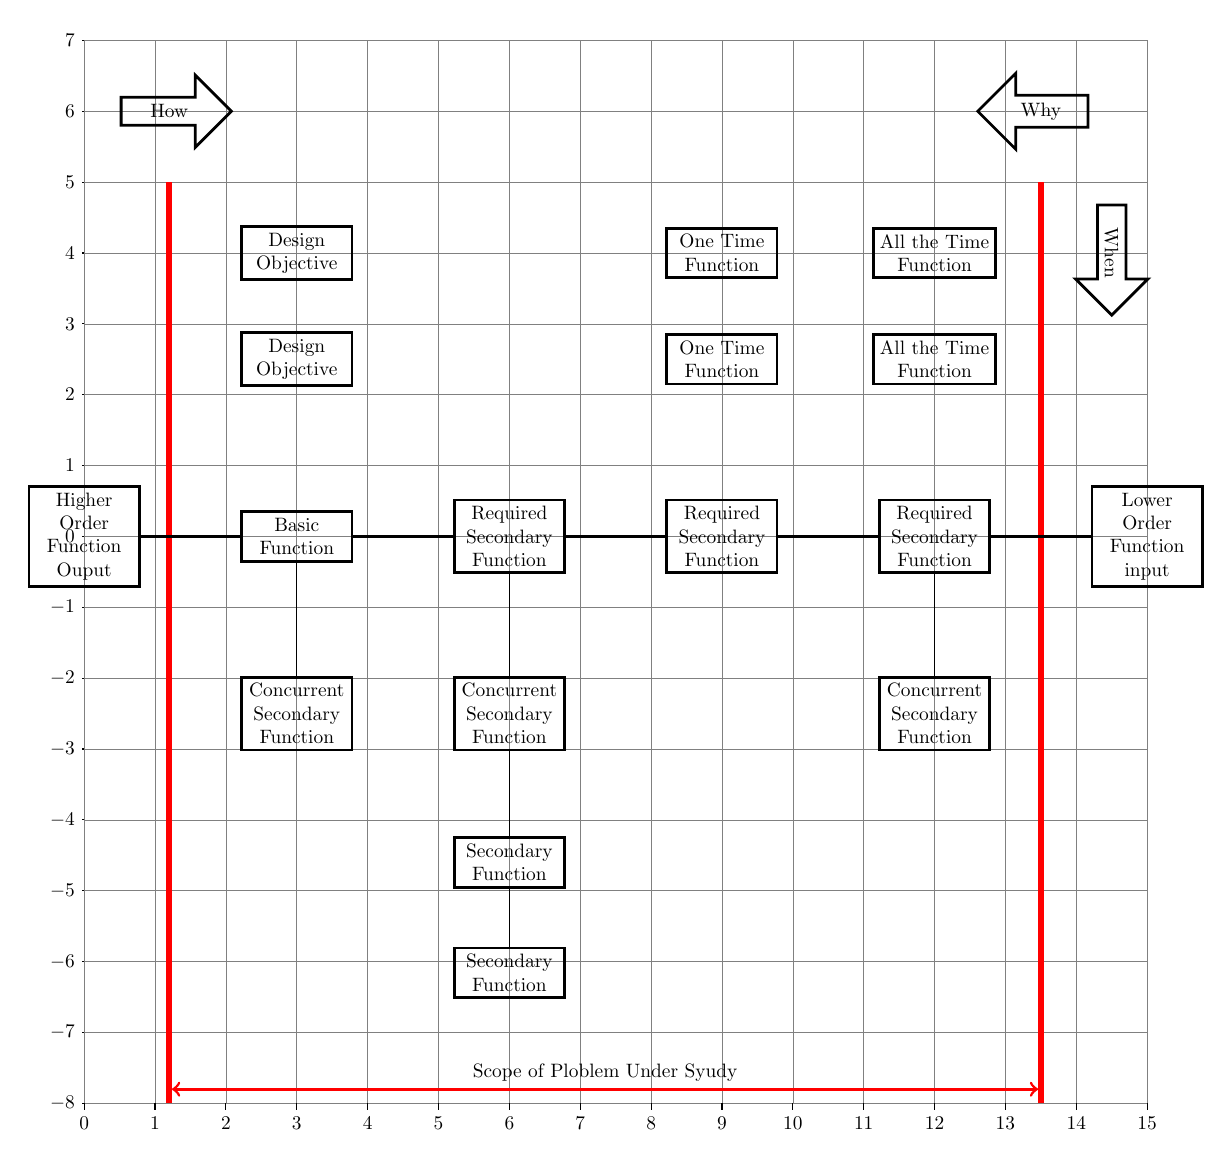
\begin{tikzpicture}[	scale=0.9, 
							every node/.style={scale=0.7},
							node distance=2.0cm,
						]
			% ---------------------------------------  draw grid
			\draw[help lines] (0,-8) grid (15,7);
			% x
			\foreach \x in {0,1,...,15}
			\draw (\x cm,-8cm) -- (\x cm, -8.1cm) node[anchor=north] {$\x$};
			% y
			\foreach \y in {-8,-7,...,7}
			\draw (0, \y cm) -- (-1pt, \y cm) node[anchor=east] {$\y$};


			\tikzstyle{block} = 	[draw, line width=1pt,
								shape=rectangle,
								align=center,
								minimum width=2.0cm,
								minimum height=1.5em,
%								text width=2cm,
								shape=rectangle,
								rounded corners=0.0em];

			\tikzstyle{rblock}=[	draw, 
								align=center,
								minimum width=3.0em,
								minimum height=1.5em,
								text width=5.0em,
								shape=rectangle,
								rounded corners=0.5em];

			% -----------------------
			\draw [red, line width=2pt] ( 1.2,5) -- (1.2,-8);
			\draw [red, line width=2pt] (13.5,5) -- (13.5,-8);
			\draw [red, line width=1pt, |<->|] (1.2,-7.8) -- (13.5,-7.8) 
				node [midway, above, black]{Scope of Ploblem Under Syudy };

			% -----------------------
			\node [	single arrow, draw,line width=1pt,
					rotate=0,
					minimum height=2cm,
					single arrow head extend=0.4cm ,
					single arrow head indent=0.0cm 
					] 
					at(1.2,6) (C00) {How};
			\node [	single arrow, draw,line width=1pt,
					shape border rotate=180,
					minimum height=2cm,
					single arrow head extend=0.4cm ,
					single arrow head indent=0.0cm 
					] 
					at(13.5,6) (C00) {Why};
			\node [	single arrow, draw,line width=1pt,
					rotate=-90,
					minimum height=2cm,
					single arrow head extend=0.4cm ,
					single arrow head indent=0.0cm 
					] 
					at(14.5,4) (C00) {When};



			\node [block] 				(B00) {Higher\\ Order\\Function \\Ouput};
			\node [block] at(3,0) 			(B11) {Basic \\Function};
			\node [block] at(6,0)		 	(B21) {Required\\Secondary\\Function};
			\node [block] at(9,0)		 	(B31) {Required\\Secondary\\Function};
			\node [block] at(12,0) 		(B41) {Required\\Secondary\\Function};
			\node [block] at(15,0) 	 	(B51) {Lower\\Order\\Function\\input};

			\draw[-,line width=1pt] (B00) -- (B11);
			\draw[-,line width=1pt] (B11) -- (B21);
			\draw[-,line width=1pt] (B21) -- (B31);
			\draw[-,line width=1pt] (B31) -- (B41);
			\draw[-,line width=1pt] (B41) -- (B51);


			\node [block] at(3,-2.5)	 	(B12) {Concurrent\\Secondary\\Function};
			\draw[-,line width=0pt] (B11) -- (B12);

			\node [block] at(6,-2.5)	 	(B22) {Concurrent\\Secondary\\Function};
			\node [block, below of=B22,yshift=-2em] 	(B23) {Secondary\\Function};
			\node [block, below of=B23,yshift=0em] 	(B24) {Secondary\\Function};
			\draw[-,line width=0pt] (B21) -- (B22);
			\draw[-,line width=0pt] (B22) -- (B23);
			\draw[-,line width=0pt] (B23) -- (B24);


			\node [block] at(12,-2.5)	 	(B42) {Concurrent\\Secondary\\Function};
			\draw[-,line width=0pt] (B41) -- (B42);


			% Design Objective
			\node [block] at(3.0, 4) 		(A01) {Design\\Objective};
			\node [block] at(3.0, 2.5)		(A02) {Design\\Objective};

			% One Time Function
			\node [block] at(9.0, 4) 		(A01) {One Time\\Function};
			\node [block] at(9.0, 2.5)		(A02) {One Time\\Function};

			% All the Time Function
			\node [block] at(12.0, 4) 		(A01) {All the Time\\Function};
			\node [block] at(12.0, 2.5)		(A02) {All the Time\\Function};
			
			\draw[-,line width=1pt] (B00) -- (B11);

		\end{tikzpicture}


































	% ==============================================================================	
	%   타이틀 페이지
	% ==============================================================================	



% ------------------------------------------------------------------------------
% Maketitle
% ------------------------------------------------------------------------------
		\begin{titlepage}
		\singlespace
		\pagestyle{empty}
		\newcommand{\HRule}{\rule{\textwidth}{0.5mm}}
		\begin{center}
		\null
		\vspace{2cm}
		\textsc{\LARGE Value Engineering}\\[1.0cm]
		\HRule\\[-0.4cm]
		\HRule \\[0.4cm]
			{ \huge \bfseries 설계의 경제성 등 검토 \\[0.4cm] }
		\HRule\\[-0.4cm]
		\HRule \\[1.5cm]
		
		% Author and supervisor
		\noindent
		\begin{minipage}{1\textwidth}
			\begin{flushright} \large \emph{Author:}  김대희	\end{flushright}
		\end{minipage}%
		\vfill
		% Bottom of the page
		{\large \today}
		
		\end{center}
		\cleardoublepage
		\end{titlepage}																						



% ------------------------------------------------------------------------------
% Maketitle
% ------------------------------------------------------------------------------
			\begin{titlepage}
			\thispagestyle{empty}				% Remove page numbering on this page
			\definecolor{grey}{rgb}{0.9,0.9,0.9} 
			\colorbox	{grey}
						{ \parbox[t]{1.0\linewidth}
						{
						\vspace*{1.2cm} 
						\fontsize{20}{20} \rmfamily \hfill \today 		\\ [0.8cm] \null
						\fontsize{40}{20} \rmfamily \hfill Value Engineering \\ [0.8cm] \null
						\fontsize{20}{50} \rmfamily \hfill ver101
						\vspace*{0.8cm} 
						} }
			\vfill
			% Print the author data as defined above
			\hfill Kim Dae Hee\\ \null
			\hfill (주)서영엔지니어링\\ \null
			\hfill 건설관리팀\\ \null
			\hfill \url{h01038395609@gmail.com} \\ \null
			\hfill \rule{0.4\linewidth}{1pt}
			\end{titlepage}
			\clearpage

% ------------------------------------------------------------------------------
% Maketitle
% ------------------------------------------------------------------------------

				\newpage   
				\thispagestyle{empty}
				\begin{center}
				\null
				\vspace{6em} % White space at the top of the page
		
				\rule{\textwidth}{1.6pt}\\[-1.9em]%\vspace{0.1pt} % Thick horizontal line
				\rule{\textwidth}{0.4pt}\\[2em]
		
				{\Huge 중점 품질 관리 대상 }\\[1.0em]
		
				\rule{\textwidth}{0.4pt}\\[-1.7em]
				\rule{\textwidth}{1.6pt}
				\end{center}



\newpage
% --------------------------------- 환경 정의 : 박스 치고 안의 글자 파란색

			\newenvironment{typing_code}
			{ 	\setlength{\fboxsep}{12pt}
				\begin{boxedminipage}[c]{1.0\linewidth}
				\color{blue}
			}
			{ 	\end{boxedminipage} 
				\color{black}
			}


			\begin{typing_code}
			code 입력
			\end{typing_code}
			

























% ------------------------------------------------------------------------------
% End document
% ------------------------------------------------------------------------------
\end{document}


